\chapter{Chapter Title} \label{c6}
\section{Figure}
\begin{itemize}
	\item All Figure Caption should be in the Title Case, TNR 10 pt, and it should be of the Format: Fig Chapter Number.Figure Number Figure Caption
	
	\item It should be cited as Fig. \ref{c6:fig1} 
	Caption must appear below the Figure.

	
	\item For Smaller: (4 Figures arranged in Two Columns) / Page; Portrait Mod.
	
	\item For Medium: (2 Figures arranged one below the other / Page; Portrait Mode.
	
	\item For Larger: 1 Figure / Page; Landscape Mode.
	
	\item Figure Label should be in Font TNR 10 pt, Bold.
	
	\item Figure Resolution should be minimum of 300 DPI.
\end{itemize}

For example, The universe is immense and it seems to be homogeneous, 
in a large scale, everywhere we look at.

	\begin{figure}[htb]
		\begin{center}
		\includegraphics[scale=0.1]{universe}
	
		\caption{Sample Picture of Universe }
		\label{c6:fig1}
	\end{center}
	\end{figure}

There's a picture of a galaxy above in Fig. \ref{c6:fig1}

\section{Graph}
Another example graph in image format is given below Fig. \ref{c6:fig2}
\begin{figure}[htb]
	\begin{center}
		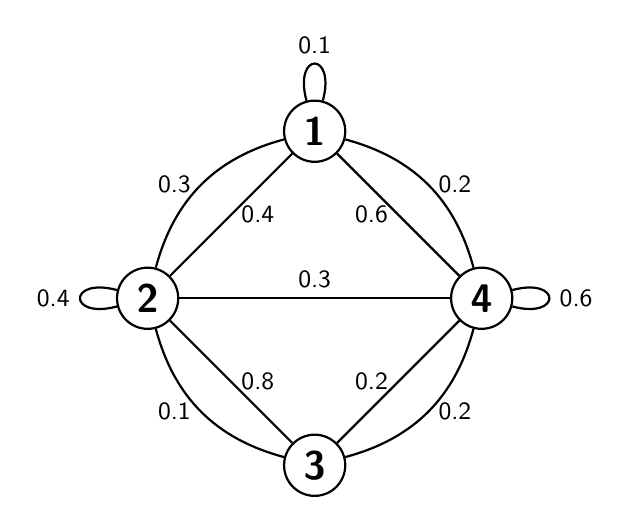
\begin{tikzpicture}[auto, node distance=3cm, every loop/.style={},
		thick,main node/.style={circle,draw,font=\sffamily\Large\bfseries}]
		
		\node[main node] (1) {1};
		\node[main node] (2) [below left of=1] {2};
		\node[main node] (3) [below right of=2] {3};
		\node[main node] (4) [below right of=1] {4};
		
		\path[every node/.style={font=\sffamily\small}]
		(1) edge node [left] {0.6} (4)
		edge [bend right] node[left] {0.3} (2)
		edge [loop above] node {0.1} (1)
		(2) edge node [right] {0.4} (1)
		edge node {0.3} (4)
		edge [loop left] node {0.4} (2)
		edge [bend right] node[left] {0.1} (3)
		(3) edge node [right] {0.8} (2)
		edge [bend right] node[right] {0.2} (4)
		(4) edge node [left] {0.2} (3)
		edge [loop right] node {0.6} (4)
		edge [bend right] node[right] {0.2} (1);
		\end{tikzpicture}
		\caption{Sample Graph}
		\label{c6:fig2}
	\end{center}
\end{figure}
